\documentclass[border={10pt, 10pt, 10pt, 10pt}]{standalone}

\usepackage{tikz}
\usepackage{graphicx}
\usepackage{varwidth}

\renewcommand\familydefault{\sfdefault}

\begin{document}
\begin{tikzpicture}

\node at (0, 0) {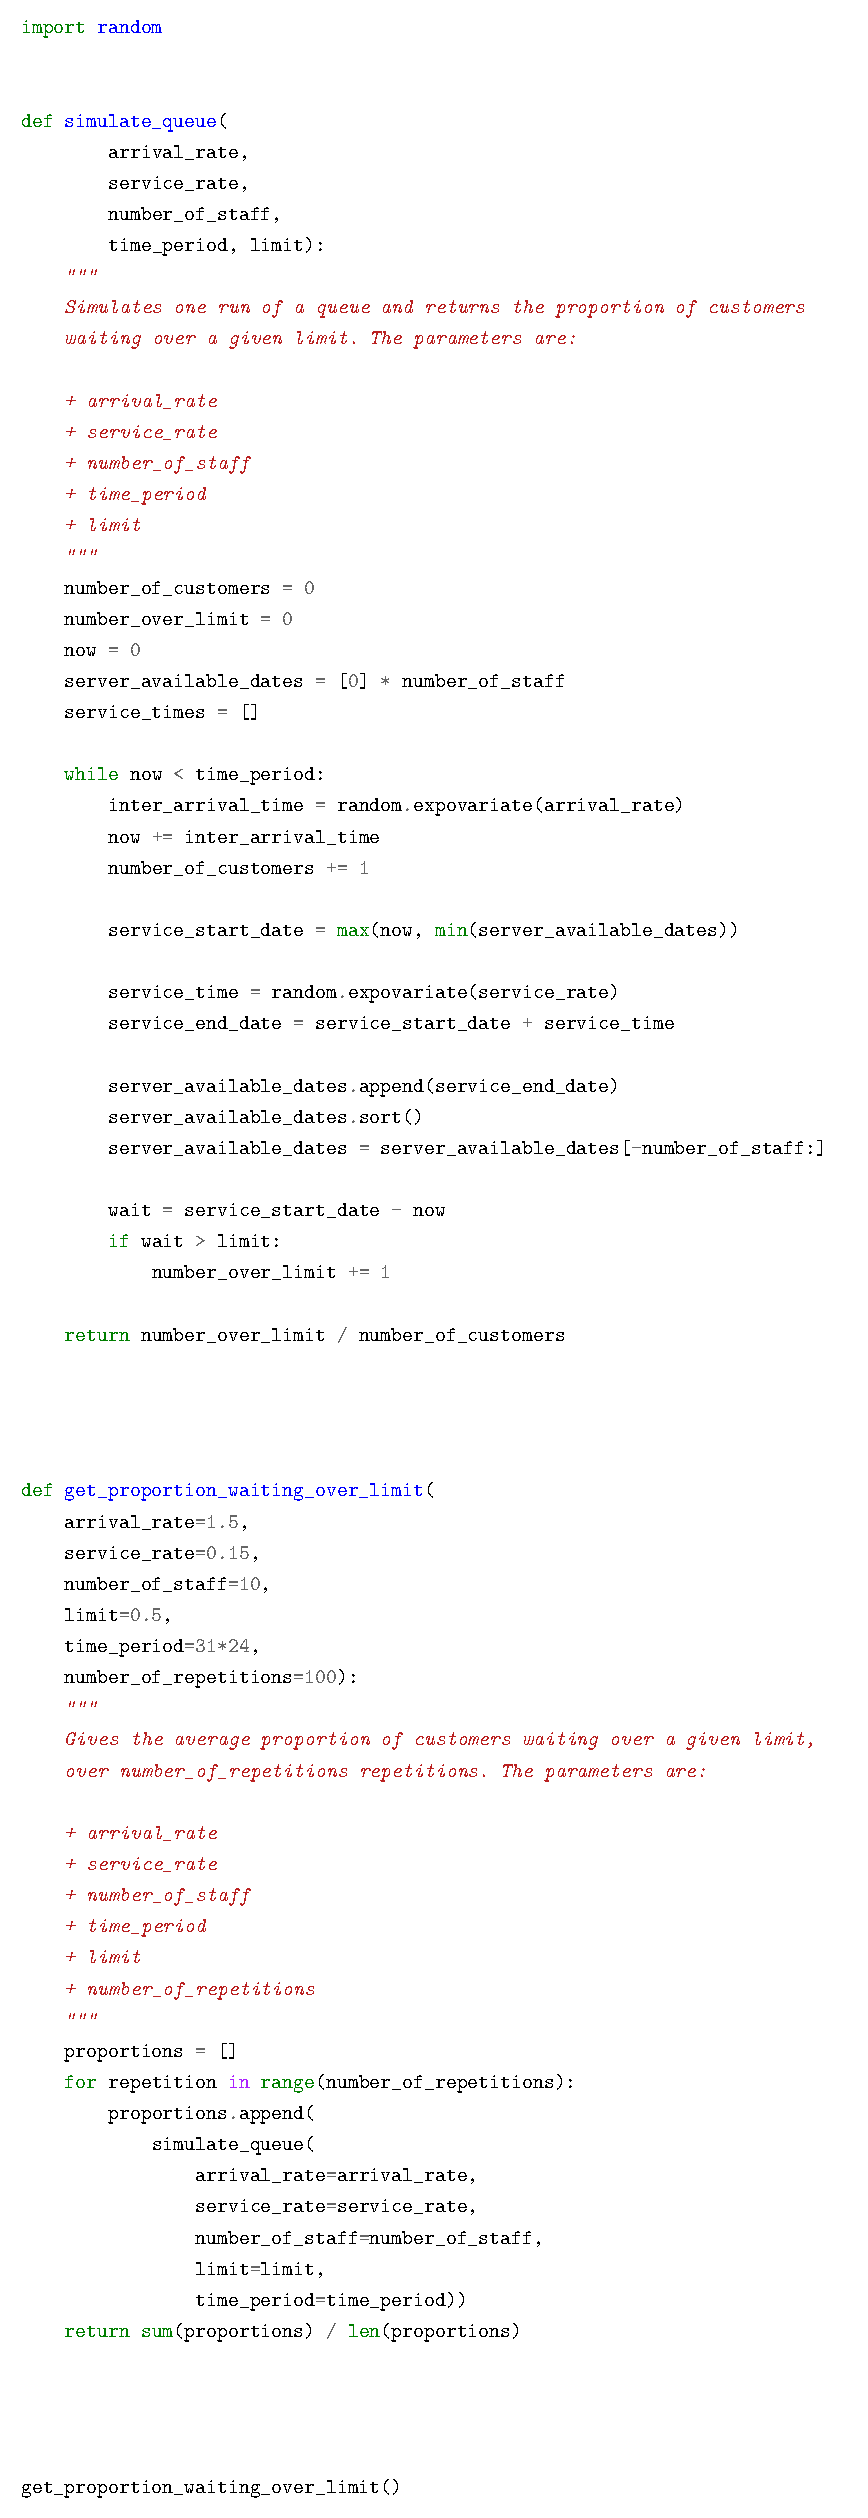
\includegraphics{concepts1.pdf}};

%%%%%%%%%%%%%
% LEFT SIDE %
%%%%%%%%%%%%%

% VARIABLES
\draw[ultra thick, draw=red!50!black] (2.5, 11.75) -- (-7.25, 11.75) -- (-7.25, 8.75) -- (2.5, 8.75);

% WHILE
\draw[ultra thick, draw=blue!50!black] (-7.25, 6) -- (-7.25, 8.5) -- (-5.5, 8.5);
\draw[ultra thick, dashed, draw=blue!50!black] (-7.25, 6) -- (-7.25, 5);
\draw[ultra thick, dotted, draw=blue!50!black] (-7.25, 5) -- (-7.25, 4);

% IF
\draw[ultra thick, draw=green!50!black] (-4.5, 0.5) -- (-7.25, 0.5) -- (-7.25, -0.5) -- (-4.5, -0.5);

% FUNCTIONS
\draw[ultra thick, draw=magenta!50!black] (-7.25, 16.5) -- (-7.25, 19.75) -- (-5, 19.75);
\draw[ultra thick, dashed, draw=magenta!50!black] (-7.25, 16.5) -- (-7.25, 15);
\draw[ultra thick, dotted, draw=magenta!50!black] (-7.25, 15) -- (-7.25, 14);

\draw[ultra thick, draw=magenta!50!black] (-7.25, -5.5) -- (-7.25, -3.5) -- (-5, -3.5);
\draw[ultra thick, dashed, draw=magenta!50!black] (-7.25, -5.5) -- (-7.25, -7);
\draw[ultra thick, dotted, draw=magenta!50!black] (-7.25, -7) -- (-7.25, -8);

\draw[ultra thick, draw=magenta!50!black] (-4.5, -20.6) -- (-7.25, -20.6) -- (-7.25, -21.1) -- (-4.5, -21.1);




%%%%%%%%%%%%%%
% RIGHT SIDE %
%%%%%%%%%%%%%%

% LISTS
\draw[ultra thick, draw=orange!50!black] (2.5, 1.35) -- (7.5, 1.35) -- (7.5, 3.35) -- (2.5, 3.35);
\draw[ultra thick, draw=orange!50!black] (-6.4, -13.1) -- (-1.5, -13.1) -- (-1.5, -13.65) -- (-6.4, -13.65);
\draw[ultra thick, draw=orange!50!black] (-6.4, -17.95) -- (3, -17.95) -- (3, -18.5) -- (-6.4, -18.5);

% FOR
\draw[ultra thick, draw=yellow!50!black] (-6.4, -13.75) -- (4, -13.75) -- (4, -17.85) -- (-6.4, -17.85);

% BOOLEANS
\draw[ultra thick, draw=cyan!50!black] (-2.5, 0.5) -- (-2.5, 0) -- (-5, 0);


%% BOXES
\draw[ultra thick, draw=red!50!black, fill=red!10!white] (-24, 21.5) rectangle (-14, 11.5);
\draw[ultra thick, draw=green!50!black, fill=green!10!white] (-24, 10.5) rectangle (-14, 0.5);
\draw[ultra thick, draw=blue!50!black, fill=blue!10!white] (-24, -0.5) rectangle (-14, -10.5);
\draw[ultra thick, draw=magenta!50!black, fill=magenta!10!white] (-24, -11.5) rectangle (-14, -21.5);

\draw[ultra thick,  draw=cyan!50!black, fill=cyan!10!white] (24, 21.5) rectangle (14, 11.5);
\draw[ultra thick, draw=orange!50!black, fill=orange!10!white] (24, 10.5) rectangle (14, 0.5);
\draw[ultra thick, draw=yellow!50!black, fill=yellow!10!white] (24, -0.5) rectangle (14, -10.5);
\draw[ultra thick, fill=black!10!white] (24, -11.5) rectangle (14, -21.5);

%% STEMS
\draw[ultra thick, draw=red!50!black] (-7.25, 10.25) -- (-8.6, 10.25) -- (-8.6, 16.5) -- (-14, 16.5); % variables
\draw[ultra thick, draw=blue!50!black] (-7.25, 7.25) -- (-11.3, 7.25) -- (-11.3, -5.5) -- (-14, -5.5); % while
\draw[ultra thick, draw=green!50!black] (-7.25, 0) -- (-12.65, 0) -- (-12.65, 5.5) -- (-14, 5.5); % if
\draw[ultra thick, draw=magenta!50!black] (-7.25, 18) -- (-9.95, 18) -- (-9.95, -16.5) -- (-14, -16.5); % functions
\draw[ultra thick, draw=magenta!50!black] (-7.25, -4.5) -- (-9.95, -4.5); % functions
\draw[ultra thick, draw=magenta!50!black] (-7.25, -20.85) -- (-9.95, -20.85) -- (-9.95, -16.5); % functions

\draw[ultra thick, draw=cyan!50!black] (-2.5, 0.25) -- (9.95, 0.25) -- (9.95, 16.5) -- (14, 16.5); % booleans
\draw[ultra thick, draw=orange!50!black] (7.5, 2.35) -- (8.6, 2.35) -- (8.6, 5.5) -- (14, 5.5); % lists
\draw[ultra thick, draw=orange!50!black] (-1.5, -13.375) -- (8.6, -13.375); % lists
\draw[ultra thick, draw=orange!50!black] (3, -18.225) -- (8.6, -18.225) -- (8.6, 2.35); % lists
\draw[ultra thick, draw=yellow!50!black] (4, -15.8) -- (11.3, -15.8) -- (11.3, -5.5) -- (14, -5.5); % for


%% TITLES/TEXT
\node[text=red!50!black] at (-19, 20.5) {\huge VARIABLES};
\node[text=green!50!black] at (-19, 9.5) {\huge IF-STATEMENTS};
\node[text=blue!50!black] at (-19, -1.5) {\huge WHILE-LOOPS};
\node[text=magenta!50!black] at (-19, -12.5) {\huge FUNCTIONS};
\node[text=cyan!50!black] at (19, 20.5) {\huge BOOLEANS};
\node[text=orange!50!black] at (19, 9.5) {\huge LISTS};
\node[text=yellow!50!black] at (19, -1.5) {\huge FOR-LOOPS};
\node[text=black!50!black] at (19, -12.5) {\huge OTHER?};


\end{tikzpicture}
\end{document}